\documentclass[a4paper,UTF8]{ctexart}

\usepackage{amsmath, amsthm, amssymb, amsfonts, hyperref, mathrsfs}%美国数学学会的包+?
\usepackage{geometry} %控制界面
\usepackage{bookmark}
\usepackage{fancyhdr} % header & footer
\usepackage{appendix} % 附录
\usepackage{tikz} %作图
\usepackage{graphicx} %插入图片的宏包
\usepackage{float} %设置图片浮动位置的宏包
%\usepackage{subfigure} %插入多图时用子图显示的宏包
\usepackage{listings} %引用代码
\usepackage{physics,mathtools} %物理数学工具
\usepackage{comment}
\usepackage{framed}
\usepackage{caption}
\usepackage{subcaption}
\geometry{top=2.5cm,bottom=2.5cm,left=2.5cm,right=2.5cm} % 布局要求
\pagestyle{fancy} % fancy分格
\fancyhf{} % 清除所有页眉页脚
\renewcommand\headrulewidth{0.6pt}
\renewcommand\footrulewidth{0.6pt}
% font
\setCJKmainfont{Noto Serif CJK SC}[BoldFont={Noto Serif CJK SC Bold}, ItalicFont=]
\lhead{何金铭 PB21020660$\mid$座位号:5}
\chead{量子计算实验预习报告}
\rhead{\thepage}
\lfoot{2024.4.12}
\rfoot{USTC}
%\bibliographystyle{plain} % 引用样式
\everymath{\displaystyle} % display
%============================================================

\begin{document}

\begin{center}
    \textbf{\Large 量子计算实验预习报告}
    \par \text{\large 何金铭 PB21020660}
\end{center}

\section{实验基本原理}

\subsection{量子比特}

一个qubit的态$\ket{\Psi} = \alpha \ket{0} + \beta \ket{1}$,可以表示成:

\begin{equation}|\Psi\rangle=cos\frac\theta2|0\rangle+e^{i\varphi}sin\frac\theta2|1\rangle.\end{equation}

可以表示为Bloch球上的一个点

\subsection{量子逻辑门}

理论上可以证明,对于任意的多比特量子逻辑门,都可以通过两比特受控非门结合单比特量子逻辑门的方式实现。我们称单比特量子逻辑门和受控非门形成一组普适的量子逻辑门

其数学上对应了$SU(2^n)$群可以用$SU(2)$的群元素来生成

\begin{figure}[H]
    \centering
    \begin{minipage}[b]{0.9\textwidth}
        \centering
        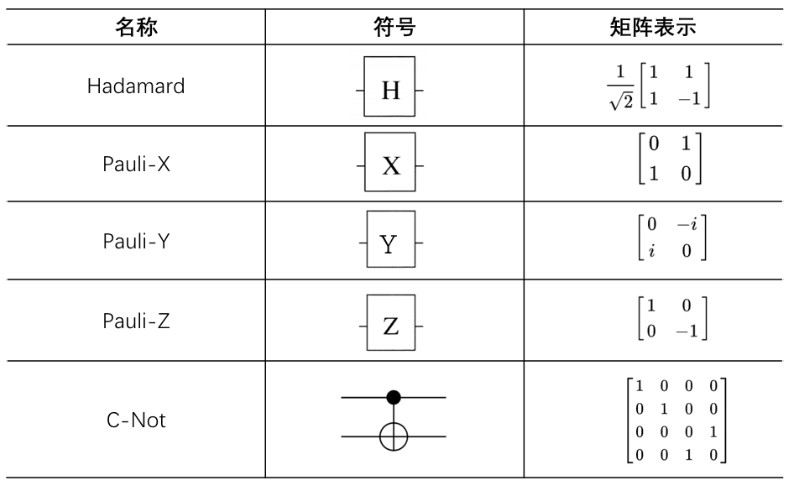
\includegraphics[width=0.9\textwidth]{./fig1.jpg}
        \caption{常用量子逻辑门的符号和矩阵表示}
    \end{minipage}
\end{figure}

\subsection{量子测量}

一个态$\ket{\Psi} = \alpha \ket{0} + \beta \ket{1}$,测量后得到的概率为$|\alpha|^2$和$|\beta|^2$

也可以选择另一组正交基$|+\rangle=\frac{1}{\sqrt{2}}(|0\rangle+|1\rangle),|-\rangle=\frac{1}{\sqrt{2}}(|0\rangle-|1\rangle)$进行测量,
测量之后,坍缩到 $|+\rangle$ 或者 $|-\rangle$ 的几率分别为 $\frac12|\alpha+\beta|^2,~\frac12|\alpha-\beta|^2$。

\subsection{量子算法}

量子算法在某些问题上有指数级的优势,比如Shor算法可以在多项式时间内分解大整数,Grover算法可以在$\sqrt{N}$时间内搜索一个无序数据库。
下面以Deutsch算法这个toy model为例,说明量子算法的优势。

函数 $f(x)$,其定义域为 {0,1},且 $f(x)\in\{0,1\}$, 那么这样的函数共有四种情
况,如下图所示:

\begin{figure}[H]
    \centering
    \begin{minipage}[b]{0.9\textwidth}
        \centering
        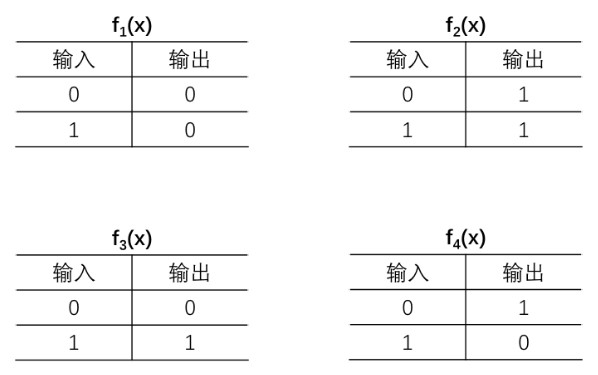
\includegraphics[width=0.9\textwidth]{./fig2.jpg}
        \caption{常函数与平衡函数举例:$f_1(x)$与$f_2(x)$是常函数,$f_3(x)$与$f_4(x)$是平衡函数。}
    \end{minipage}
\end{figure}

现在我们需要判断 $f(x)$ 是常函数还是平衡函数,采用经典计算的方法,
需要分别计算 $f(0)$ 和 $f(1)$,然后判断 $f(0)$ 和 $f(1)$ 是否相等,
共需进行两次计算。如果采用量子计算中的 Deutsch 算法,
则只需一次计算就能够判定。如下图所示,是Deutsch 算法的量子线路图。
该量子算法需要两个量子比特,其初态是 $|a\rangle=|01\rangle$


\begin{figure}[H]
    \centering
    \begin{minipage}[b]{0.9\textwidth}
        \centering
        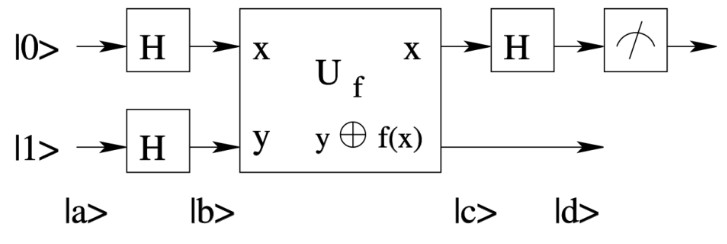
\includegraphics[width=0.9\textwidth]{./fig3.jpg}
        \caption{Deutsch算法的量子线路图}
    \end{minipage}
\end{figure}

经过计算可得:

\begin{itemize}
    \item 若 $f(x)$ 是常函数,则$|d\rangle=\pm|0\rangle(\frac{|0\rangle-|1\rangle}{\sqrt{2}})$,测量结果为 $0$;
    \item 若 $f(x)$ 是平衡函数,则$|d\rangle=\pm|1\rangle(\frac{|0\rangle-|1\rangle}{\sqrt{2}})$,测量结果为 $1$。
\end{itemize}

总结一下 Deutsch 算法的过程,我们将量子比特制备到 $\left|0\right>$ 和 $\left|1\right>$ 的叠加态,只需进行一次计算,就可以根据末态的测量结果是 0 还是 1, 来判断 f(x) 是常函数还是平衡函数。根据经典算法,则需进行两次计算。将 Deutsch 算法的定义域从 $\{0,1\}$ 推广到 $\{0,1\}^n$, 其解决方法即是 D-J 算法。D-J 算法是最早提出的量子算法之一, 虽然 D-J 算法解决的问题不具备太多实际意义,但该算法向人们展示了,解决某些问题时,量子计算能够比经典计算更高效。下面我们将讨论如何在实验上实现这一算法。

\section{实验具体实现}

\subsection{DiVincenzo判据}

2000 年,DiVincenzo 讨论了实现量子计算的物理要求,并提出了如下的 7 条判
据:

\begin{enumerate}
    \item 可扩展的具有良好特性的量子比特系统;
    \item 能够制备量子比特到某个基准态;
    \item 具有足够长的相干时间来完成量子逻辑门操作;
    \item 能够实现一套通用量子逻辑门操作;
    \item 能够测量量子比特;
    \item 能够使飞行量子比特和静止量子比特互相转化;
    \item 能够使飞行量子比特准确地在不同的地方之间传送。
\end{enumerate}

后面两条是针对量子计算机之间通信提出的要求,前面五条是实现量子计算的要求。

\subsection{金刚石中的NV色心}

NV (Nitrogen-Vacancy) 色心是金刚石中的一种点缺陷。金刚石晶格中一个碳原子缺失形成空位,近邻的位置有一个氮原子,这样就形成以了一个 NV 色心。我们这里所说的 NV 色心,指的是带负电荷 $NV^-$ 顺磁中心。NV 色心的有六个电子, 两个来自氮原子,三个来自与空位相邻的碳原子,另外一个是俘获的 (来自施主杂质的) 电子。

\begin{figure}[H]
    \centering
    \begin{minipage}[b]{0.9\textwidth}
        \centering
        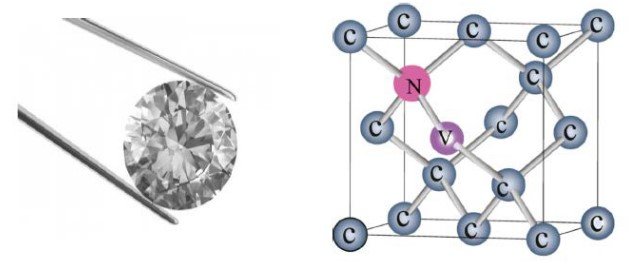
\includegraphics[width=0.8\textwidth]{./fig4.jpg}
        \caption{金刚石和金刚石中的NV色心原子结构}
    \end{minipage}
\end{figure}




\subsection{自旋态初始化和读出}

\begin{figure}[H]
    \centering
    \begin{minipage}[b]{0.9\textwidth}
        \centering
        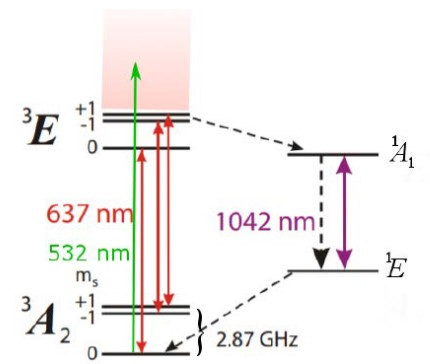
\includegraphics[width=0.6\textwidth]{./fig5.jpg}
        \caption{室温下金刚石NV色心的能级结构示意图。会辐射出光子的跃迁用实线箭头表示,非辐射跃迁用虚线箭头表示}
    \end{minipage}
\end{figure}

上图是室温下金刚石 NV 色心的能级结构。NV 色心的基态为自旋三重态,三重态基态与激发态间跃迁相应的零声子线为 637 nm, 红色区域为声子边带。基态的自旋三重态 ($|m_s=0\rangle,|m_s=1\rangle,|m_s=-1\rangle)$ 中,$|m_s=1\rangle,|m_s=-1\rangle$ 在无磁场时是简并的,它们与$\left|m_s=0\right\rangle$态之间的能隙 (零场劈裂) 对应微波频率为 2.87 GHz。激发态的能级自旋分裂对应的微波频率为 1.4 GH$z$。

首先 532 nm 的激光激发基态电子,由于电子跃迁是电偶极跃迁与电子自旋无关,所以跃迁前后的自旋是守恒的。$|m_s=0\rangle$ 的基态电子到 $|m_s=0\rangle$ 的声子边带, 而 $|m_s=\pm1\rangle$ 的基态电子到 $|m_s=\pm1\rangle$ 的声子边带。之后 $|m_s=0\rangle$ 的电子绝大多数都直接跃迁到基态辐射荧光,而$|m_s=\pm1\rangle$ 的电子则有一部分直接跃迁到基态辐射荧光,而另一部分通过无辐射跃迁到单重态再到三重态的$\left|m_s=0\right>$态。经过多个周
期之后,基态$|m_s=\pm1\rangle$上的布居度会越少越少,
而$|m_s=0\rangle$上的布居度会越来越多。这相当于,在激光的照射下,
布居度从 $|m_s=\pm1\rangle$ 转移到了 $|m_s=0\rangle$, 
从而实现了自旋极化。温下 NV 色心电子自旋的极化率可达 95$\%$以上。

如果我们选取基态的$\left|m_s=0\right\rangle$和$\left|m_s=1\right>$作为量子比特,NV 色心的自旋极化就对应于将量子比特的初态极化到 $\left|0\right>$ 态。

由于 $|m_s=\pm1\rangle$ 态有更大的概率通过无辐射跃迁,回到基态。
所以 $|m_s=0\rangle$ 态的荧光比 $|m_s=\pm1\rangle$ 态的荧光强度大,
实验上得出大约大 20-40$\%$。根据 $|m_s=0\rangle$ 态
和$|m_s=\pm1\rangle$ 对应荧光强度的差别,就可以区分 NV 色心的自旋态,
即实现对自旋量子比特状态的读出。由于由于单次实验得到的 $|m_s=0\rangle$ 态
和 $|m_s=\pm1\rangle$ 的荧光强度并不明显,室温下对 NV 色心电子自旋量子比特
的测量一般为多次实验重复测量, 测得的结果为某个观测量 
(如 $|m_s=0\rangle\langle m_s=0|)$ 的平均值。

\subsection{自旋态操控}

\begin{figure}[H]
    \centering
    \begin{minipage}[b]{0.9\textwidth}
        \centering
        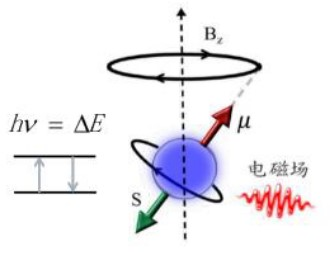
\includegraphics[width=0.4\textwidth]{./fig6.jpg}
        \caption{自旋磁共振原理示意图}
    \end{minipage}
\end{figure}

一个自旋系统$\vec\mu=\gamma\vec{S}=\gamma\frac{\hbar}{2}\vec{\sigma}$
在外场$\vec B$的作用下,会根据系统哈密顿量进行演化:$H=-\vec{\mu}\cdot\vec{B_0}$

\subsubsection{自旋进动}

在外场$\vec B$的作用下,自旋会进动,进动频率为$\omega=\gamma B_0$

\begin{equation}\begin{gathered}
\langle S_z\rangle=\frac{\hbar}{2}cos\alpha; \\
\langle S_{x}\rangle=\frac{\hbar}{2}sin\alpha cos(\omega_{0}t+\alpha_{0}); \\
\langle S_{y}\rangle=-\frac{\hbar}{2}sin\alpha sin(\omega_{0}t+\alpha_{0}); 
\end{gathered}\end{equation}

对于上述结果,可以有一个直观的几何解释。如下图所示,磁矩的 XY 分量大小是 $\frac12\hbar sin\alpha$,并且绕着外磁场方向 Z 轴转动,转动频率为 $\omega_0$。这个过程也叫作拉莫进动,$\omega_0$ 被称作拉莫频率。

\begin{figure}[H]
    \centering
    \begin{minipage}[b]{0.9\textwidth}
        \centering
        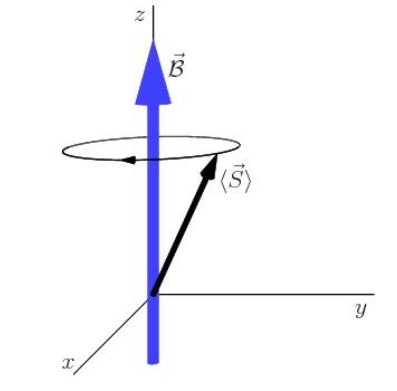
\includegraphics[width=0.4\textwidth]{./fig8.jpg}
        \caption{磁矩绕着外磁场方向做拉莫进动}
    \end{minipage}
\end{figure}

\subsubsection{共振微波驱动}

\begin{figure}[H]
    \centering
    \begin{minipage}[b]{0.9\textwidth}
        \centering
        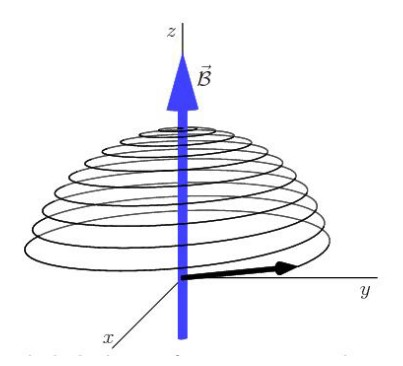
\includegraphics[width=0.4\textwidth]{./fig9.jpg}
        \caption{微波频率与拉莫进动频率一致时,磁矩绕着外磁场方向z轴做章动}
    \end{minipage}
\end{figure}

考虑在施加一个 XY 平面内圆偏振的微波场:

$$
\left\{\begin{array}{l}B_x=B_1cos\omega t\\[1ex]B_y=B_1sin\omega t\end{array}\right.
$$


通过求解薛定谔方程,可以得到:

$$
P_\uparrow=|a(t)|^2=\frac{\omega_1^2}{\omega_1^2+(\omega_0-\omega)^2}sin^2\delta t.
$$
其中,
$$
\delta=\sqrt{\omega_1^2+(\omega_0-\omega)^2}.
$$

该过程也可以几何的理解。前面提到,当有静磁场的时候,自旋绕着静磁场方向做进动。当施加一个额外交变磁场,自旋会感受一个力矩,使其从 $z$ 轴向 $-z$ 轴方向翻转。这个过程也叫作自旋的拉比振荡,翻转频率也称作拉比频率。

\begin{figure}[H]
    \centering
    \begin{minipage}[b]{0.9\textwidth}
        \centering
        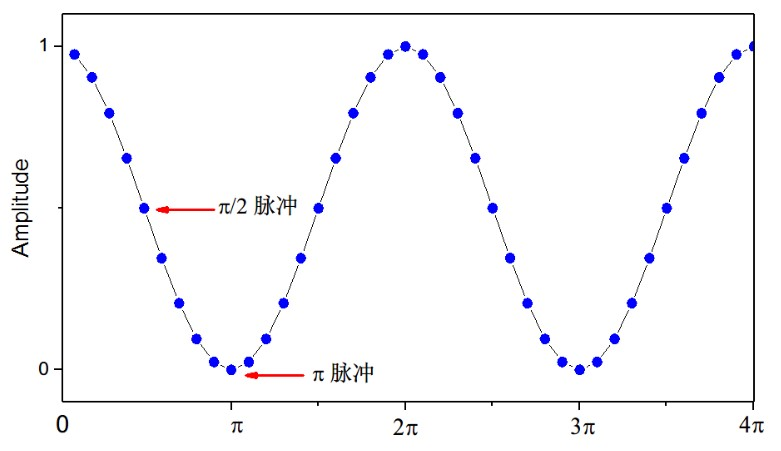
\includegraphics[width=0.8\textwidth]{./fig10.jpg}
        \caption{拉比振荡曲线示意图}
    \end{minipage}
\end{figure}

实现了拉比振荡,即说明实现了对 NV 色心自旋的相干操控,量子比特在 $|0\rangle$ 态和 $|1\rangle$ 态之间振荡。共振驱动的情况下,当 $\omega_1t=\pi$ 时,量子比特从 $|0\rangle$ 态完全转到了 $|1\rangle$ 态,即实现了一个非门操作,这个脉冲也叫作 $\pi$ 脉冲。当 $\omega_1t=\frac\pi2$ 时,我们得到 $|0\rangle$ 态和 $|1\rangle$ 的叠加态,即 $|0\rangle\to\frac{|0\rangle+i|1\rangle}{\sqrt{2}}$。这是量子计算中非常重要的逻辑门, 这个脉冲也叫作 $\frac\pi2$ 脉冲。

\subsection{实验装置}

\begin{figure}[H]
    \centering
    \begin{minipage}[b]{0.9\textwidth}
        \centering
        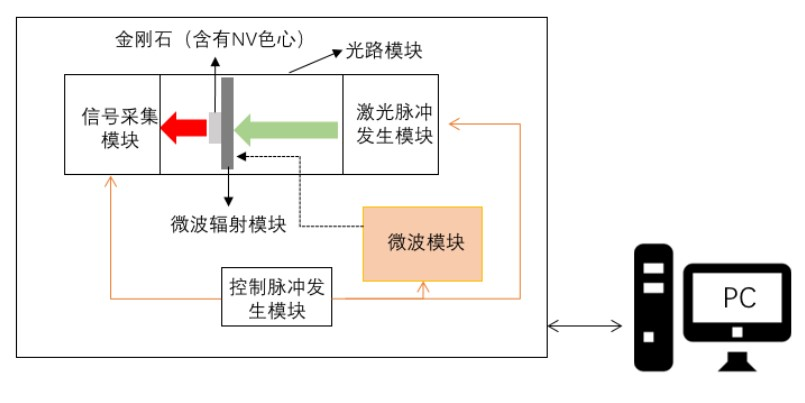
\includegraphics[width=0.9\textwidth]{./fig7.jpg}
        \caption{实验装置图}
    \end{minipage}
\end{figure}

\subsubsection{光学模块}

上图中的激光发生模块,光路模块和信号采集模块统称光学模块。激光脉冲发生模块产生 532 nm 的绿色激光脉冲,用于 NV 色心状态的初始化和读出。光路模块将绿色的激光聚焦到金刚石上,金刚石中的 NV 色心在绿色激光的照射下,会发出红色荧光。在金刚石之后,经过滤波,再将荧光聚焦到光电探测器中。光电探测器将光信号转化成电信号,发送给信号采集模块。

\subsubsection{微波模块}

前面提到,对于 NV 色心自旋状态的操控,是通过施加微波脉冲实现的。微波模块中,微波源产生特定频率的微波信号,经过微波开关调制成脉冲形式,然后经过微波功率放大器,实现功率增强。最后进入微波辐射模块,辐射到金刚石上。

\subsubsection{控制脉冲发生模块}

控制脉冲发生模块,负责产生TTL信号,输送给微波模块、激光脉冲发生模块和信号采集模块。一方面,用于触发微波开关和激光器的输出,调制微波脉冲和激光脉冲。另一方面,用于同步各个不同器件之间的时序

\section{实验内容}

\subsection{连续波实验}

测量 NV 色心连续波谱的时候,收集的是其发出的荧光信号,这其中的物理基础是,NV 色心的自旋态能够被激光初始化,并且发出荧光的亮度是依赖于自旋状态
 的。施加微波到色心上,可以改变自旋在 $|m_s=0\rangle$ 态和 $|m_s=\pm1\rangle$ 态的布居,从而改变荧光强度。因为 NV 色心的荧光亮度是依赖于自旋态的。改变施加的微波频率, 当共振的微波改变了自旋状态,荧光亮度会相应的发生改变。因此,但微波频率与能级间隔共振时,谱线上会出现低谷。


\subsection{拉比振荡实验}

对于 NV 色心而言,实现拉比振荡的脉冲序列如下:首先打开激光,将 NV 色心自旋态初始化到 $\left|m_s=0\right>$,然后关闭激
光,打开微波。微波脉冲的频率等于共振频率,最后再施加激光,将 NV 色心自旋态读出。施加的微波脉冲宽度不同,自旋演化的状态就不同。将微波脉冲宽度与荧光计
 数对应起来,就可以得到拉比振荡的曲线。本实验中需要用到 $|m_s=0\rangle\to|m_s=1\rangle$ 和 $|m_s=0\rangle\to|m_s=-1\rangle$ 两个跃迁频率,所以微波模块中有个两个微波源,在进行拉比振荡实验的时候,用两个波源 (记为“波源 1”和“波源 2”) 分别测定两个频率的拉比振荡。


\subsection{回波实验}

在磁共振实验中,回波实验是指,通过施加去耦脉冲的方式,让自旋相干信号重聚的过程。图 3.5所示是回波实验的脉冲序列。首先用激光将 NV 色心自旋态初始化到$|m_s=0\rangle$态,然后施加$\frac\pi2$ 脉冲,将自旋制备到 $|0\rangle$ 态和 $|1\rangle$ 态的叠加态,自由演化时间 $\tau=t1$ 后,施加 $\pi$ 脉冲,然后再等待自由演化时间 $\tau=t$, 施加第二个 $\frac\pi2$ 脉冲,将相干信息转化成布居度读出。

\subsection{$T_2$实验}

$T_{2}$ 实验,也叫作自旋回波实验,其目的是测量 NV 色心自旋的退相干时间。因为量子系统不是一个孤立系统,其与环境的相互作用,会引起退相干效应。图 3.7所示是 $T_{2}$ 实验的脉冲序列。首先用激光将 NV 色心自旋态初始化到 $|m_s=0\rangle$ 态,然后施加 $\frac\pi2$ 脉冲,将自旋制备到 $|0\rangle$ 态和 $|1\rangle$ 态的叠加态,自由演化时间 $\tau=\frac t2$ 后,施加$\pi$ 脉冲,然后再等待自由演化时间 $\tau=\frac t2$, 施加第二个 $\frac\pi2$ 脉冲,将相干信息转化成布居度读出。

\subsection{D-J算法实验}

我们将量子比特和辅助比特均编码到 $S=1$ 的电子自旋上。$U_f(x)$ 的定义与公式 1.8一致,即 $U_f(x)=(-1)^{f(x)}|x\rangle$,其中$\mathrm{f( x) }$ 表示四个不同的函数,$f_1(x)=0$ 和 $f_2(x)=1$ 是常函数,$f_3(x)=f_4(x)=1-x$ 是平衡函数,其输入输出情况如图 1.4所示。对于两能级体系,$U_{fi}$ 的矩阵表示见图 3.10。实现量子算法时,我们将 $|0\rangle$ 和 $|-1\rangle$ 编码成量子比特,$|1\rangle$ 为辅助能级。在系统用激光初始化到 $|0\rangle$ 后,输入态用 MW1 的 $\frac\pi2$ 脉冲作用在 $|0\rangle$ 上而制备得到。控制门 ($U_{fi}$) 通过 2$\pi$ 脉冲的四种组合实现。当 MW2 的 2$\pi$ 微波脉冲作用在辅助
态 $|1\rangle$ 上时,会在 $|0\rangle$ 上产生 $\pi$ 相位,等效于 $|0\rangle$ 和 $|-1\rangle$ 张成的子空间进行绕 z 轴的 $\pi$ 旋转。常函数作用结束后,末态是 $\pm\frac{|0\rangle+|1\rangle}{\sqrt{2}}$。平衡函数作用结束后,末态是士$\frac{|0\rangle-|1\rangle}{\sqrt{2}}$。两种未态分别对应正向的回波,和反向的回波。因此,我们就以通过回波测量,来判断$U_{fi}$ 操作对应的是常函数还是平衡函数。

\end{document}